% !TeX spellcheck = en_US
\documentclass[11pt, fleqn, titlepage]{article}
%\usepackage{siunitx}
\usepackage{texfiles/SpeedyGonzales}
\usepackage{texfiles/MediocreMike}
\newcommand{\so}[2]{{#1}\mathrm{e}{#2}}
% \geometry{top=1cm}
\usepackage{hyperref}
\usepackage{amsmath}
\usepackage{ragged2e}
\usepackage{booktabs}
\usepackage{lipsum}
\usepackage{csquotes}
\usepackage{longtable}
\usepackage{arydshln}
\hypersetup{
	colorlinks=true,
	linkcolor=blue,
	filecolor=magenta,      
	urlcolor=cyan,
}
\usepackage{subfig}
\usepackage{graphicx}
\title{Fairness in Classification}
\author{Anders Henriksen \\ Oskar Eiler Wiese Christensen  \\ \texttt{\{s183917, s183904\}@student.dtu.dk}}
\date{\today}

\pagestyle{plain}
\fancyhf{}
\rfoot{Page \thepage{} of \pageref{LastPage}}

\graphicspath{{Billeder/}}

\begin{document}
	
	\maketitle
	\begin{abstract}
		\textbf{TODO: Skal indeholde motivation, problem, fremgangsmåde, resultater og konklusion.} \\ \lipsum[1-2]
	\end{abstract}
	\tableofcontents \newpage
	%\thispagestyle{fancy}
	%\tableofcontents	
	
	\section{Introduction} \label{indledning}
	\textbf{TODO: \\ Hvad er formålet med projektet? \\ Hvad er problemformuleringen \\ Hvad er state-of-the-art? \\ Hvilken fremgangsmåde bruges til at løse problemet? \\ Hvem har brug for resultaterne?}
	
	\subsection{Motivation}
	Artifical intelligence (AI) and machine learning (ML) methods are playing a bigger and bigger role in modern society. As the accuracies of AI and ML models increase, their applications become wider, allowing for these  models to be implemented either as ground truth or as a pointer in applications like autonomous vehicles, medical imaging, the American judicial system ect. These models are, for the general public, often seen as an objective decision maker. As such, it becomes of essence to avoid discrimination, since model discrimination could lead to reinforced societal discrimination. Bias seems to originate from the dataset, meaning that a saving grace would be to either implement bias correction on the dataset to remove the bias from the source of the problem or to remove bias from the model, thereby removing the risk of discrimination when using the model for classification tasks. This report aims to understand bias and how it affects datasets as well as classification models. Furthermore, a set of bias correction methods will be put to use in order to explore the possibilites of keeping discrimination away from important fields. More specifically, the questions to be answered throughout the report are whether there is a bias in the COMPAS recidivism dataset and which kind of bias there is, as well as what this bias means in the dataset. Meanwhile, it is also analyzed how bias affects a classification algorithm, how bias in an algorithm is detected and how to quantify the bias. Lastly, bias correction methods will be implemented and tested and an ethical discussion will be carried out to understand the applications of bias correction algorithms and AI models on society as well as how society can learn to trust these models. \\
	
	\noindent In this report, the rest of section \ref{indledning} will focus on state of the art within the field of bias correction and the contributions from this report. Afterwards, section \ref{data} will present the necessary details of the data including visualizations of the data, explanations of the variables of the dataset and how the data came to be. Section \ref{methods} on methods sets up the necessary background knowledge for the topics of FFNNs, bayesian optimization and permutation tests. Results will be illustrated in section \ref{results} through figures and tables, which will then be discussed and put into a greater perspective in section \ref{discussion}. The discussion also contains the ethical discussion of bias and bias correction as a whole. The whole report will be summed up in section \ref{conclusion}. Some lesser relevant figures and points have been left out of the report but can be found in section \ref{appendix} and the relevant sources are found in section \ref{bibliography}
	
	\subsection{State of the Art}
	There are currently two main ways to ensure fairness in classification. One is by implementing steps during the training process of the classifier, and the second involves steps post-processing. Many different suggestions of how to implement bias correction algorithms within the field of fair AI have been proposed. 
	
	An approach proposed by Zafar et al. \cite{Zafar}, suggests that a way to achieve fair classifiers is by using linear constraints on the covariance between predicted labels and the value of features. This is a method that is implemented during the training process. "Satisfying Real-world Goals with Dataset Constraints" uses this same tactic to remove bias from the dataset. They propose that by implementing constraints in the training data, and by using the ramp penalty to quantify cost accurately, they succeed in developing an efficient algorithm to optimize the resulting non-convex constrained optimization problem. This state of the art algorithm can be implemented in situations where one may require a classifier to make prediction with a certain rate of positive predictions in order to maintain fairness for a population. \cite{g_goh} \\
	
	\noindent The main method that will be demonstrated in this project is proposed by Hardt et al. \cite{equal_of_oppor}. The suggested method can achieve a non-discriminatory classifier by post-processing the estimators of probability for a discriminant classifier to learn thresholds in order to deal with sensitive features or groups in the data. The method requires that the classifier has information about the data at decision-time, which is the case in the experiment conducted in this project. The idea is to first train an unfair classifier on the COMPAS data-set and then using post hoc correction to correct the classifier. However, another article, namely "Learning Non Discriminatory Predictors", argue that by only using the post hoc correction, the algorithm will still be unfair. They show that for several loss-functions such as the 0-1 or hinge loss, the method proposed by Hardt et al. \cite{equal_of_oppor} can fail. Despite if the Bayes optimal predictor with respect to those losses is learned	in the first step. In the paper, a notion is defined to obtain an approximation of a non-discrimination algorithm. However, this notion is explored during the paper, and it turns out that creating a non-discrimination algorithm is computationally hard. Therefore, a relaxation definition of equalized odds is presented, which is based on a second-moment condition instead of full conditional independence. Throughout the paper, it is shown that under this condition it is possible to learn a nearly optimal non-discriminatory linear predictor with respect to a convex loss without it being too computational to train. \cite{b_woodworth}
	
	
	\subsection{Contributions}
	This report aims to give an approachable account of the effect of bias as well as the most promising methods of removing bias and avoiding discrimination from learned supervised learning models in datasets. As such, the reader can expect to get the following from this report.
	
	\begin{itemize}
		\item The effects of bias in data
		\item Comprehensive guide to COMPAS data variables
		\item Bias correction methods
		\item ethical discussion of bias and discriminating models
		
	\end{itemize}
	
	
	\section{Data} \label{data}
	\textbf{TODO: \\ Data kan kort introduceres i indledningen \\ Lav etisk diskussion om opbevaring af data samt privacy issues}
	
	\noindent To analyse the efficacy of using bias correction to remove discrimination among races in the American justice system, the modified COMAS recidivism dataset from ProPublica has been used. \\
	A general overview of the dataset and how it came to be as well as the variables used for the classifier is given in \ref{dataDescription}. The data and variables have not been properly explained to any extent in examined literature, so \ref{dataExamination} will cover the meaning of all 53 variables of the dataset to remove ambiguity and set a common ground from which to base the future analysis. Lastly, \ref{dataVisuals} will show important visualizations of features of the dataset to cover which of the variables are most likely to contain biases that will be explored further in later sections.
	
	\subsection{Description of Data} \label{dataDescription}
	The data used in this project stems from an initial analysis of the COMPAS (Correctional Offender Management Profiling for Alternative Sanctions) algorithm by its developers, Northpointe Inc. After this analysis, ProPublica made a subsequent analysis of this data as well as their own queries of the offenders involved and data of the offenders who actually recidivated. This data is stored in the \texttt{compas-scores-two-year.csv} dataset from ProPublica's GitHub page, which can be found here: \url{https://github.com/propublica/compas-analysis/blob/master/compas-scores-two-years.csv}. \\\\
	\noindent The data consists of 53 different variables, 9 of which are used in the binary classification model. Four of the chosen variables are categorical, so these will have to be one-out-of-k encoded to be able to feed the necessary variables into the neural network. Meanwhile, the numerical variables, of which there are also four, will be normalized as to avoid the vanishing gradient problem and to avoid having some variables be of more importance to the final prediction. This will be explained more thoroughly in \ref{Feed-forward neural}. \\
	The 10 chosen variables, of which one will be used as the target variable are shown and explained below. To see an exhaustive explanation of all variables from the full dataset, see \ref{dataExamination}.
	
	
	\begin{table}[H]\label{resultater}
		\centering
		\begin{tabular}{l l l}
			Variable & Description & Type \\ \hline
			age & The age of the offenders & Continuous ratio \\
			priors\_count & The number of previous offences & Discrete interval \\
			juv\_fel\_count & The number of previous juvenile felonies & Discrete interval \\
			juv\_misd\_count & The number of previous juvenile misdemeanor & Discrete interval \\
			c\_charge\_degree & The severity of the offence & Discrete nominal \\
			race & The race of the offender & Discrete nominal \\
			age\_cat & The age category of the offender & Discrete nominal \\
			sex & The sex of the offender & Discrete nominal \\
			score\_text & The COMPAS prediction of chance of recidivism & Discrete interval
		\end{tabular}
		%\caption{text}
	\end{table}
		
		
	\subsection{Explanation of Data Variables} \label{dataExamination}
	To remove ambiguity about the meaning of the variables in the COMAS recidivism dataset, an exhaustive description of every variable and variable type has been produced. This allows for the results of this report to be contained within this interpretation and shines light on the true contents of the dataset, as no one else has done this before. Some variables, mostly those with \textit{c\_}, \textit{r\_} or \textit{vr\_} prefixes,have been grouped together in the table, as these serve the same purpose in the dataset for \textit{custody}, \textit{recidivism} and \textit{violent recidivism} cases respectively. 
	
	\noindent Some variable names have the prefix \textit{v\_}, which has been disregarded as an error. As such, this interpretation of the dataset assumes that these variables are akin to those with the \textit{vr\_} prefix, representing the variables related to violent recidivism. Furthermore, in the case of a few of the variables in the dataset, it has simply not been possible to find a meaningful interpretation, since the entire column is either full of NaN's like in the case of \textit{violent\_recid} or every value of the column one to one with another variable, which is the case between \textit{decile\_score} and \textit{decile\_score\_1} as well as \textit{priors\_count} and \textit{priors\_count\_2}. These variables are kept in the table for completeness but seem to have no discernible purpose in the dataset.
	
	
	\begin{longtable}{l l l} \label{allVars}
		\centering
		Variable & Description & Type \\ \hline
		id & Index of the column & Discrete interval \\
		name & Full name of the offender & Discrete nominal \\
		first & First name of the offender & Discrete nominal \\
		last & Last name of the offender & Discrete nominal \\
		compas\_screening\_date & The date the COMAS score was given & Discrete nominal \\
		sex & The sex of the offender & Discrete nominal \\
		dob & The offender's date of birth & Discrete nominal \\
		age & The offender's age & Continuous ratio \\
		age\_cat & Which age category the offender belongs to & Discrete nominal \\
		race & The offender's race & Discrete nominal \\
		juv\_fel\_count & The number of previous juvenile felonies & Discrete interval \\
		juv\_misd\_count & The number of previous juvenile misdemeanor & Discrete interval \\
		juv\_other\_count & The other types of previous juvenile crimes & Discrete interval \\
		days\_b\_screening\_arrest & ----- & Discrete interval \\ \hdashline
		priors\_count & The number of previous offences & Discrete interval \\
		priors\_count\_2 & & \\ \hdashline
		c\_jail\_in & The date the offender was jailed & Discrete nominal \\
		r\_jail\_in & & \\ \hdashline
		c\_jail\_out & The date the offender was removed from jail & Discrete nominal \\
		r\_jail\_out & & \\ \hdashline
		c\_case\_number & The offense case number & Discrete nominal \\
		r\_case\_number & & \\
		vr\_case\_number & & \\ \hdashline
		c\_offense\_date & The date the offense was performed & Discrete nominal \\
		r\_offense\_date & & \\
		vr\_offense\_date & & \\ \hdashline
		c\_charge\_degree & The severity of the offense & Discrete nominal \\
		r\_charge\_degree & & \\
		vr\_charge\_degree & & \\ \hdashline
		c\_charge\_desc & The offense that was performed & Discrete nominal \\
		r\_charge\_desc & & \\
		vr\_charge\_desc & & \\ \hdashline
		c\_arrest\_date & ----- & Discrete nominal \\
		c\_days\_from\_compas & ------ & Discrete interval \\
		r\_days\_from\_arrest & Recidivism days until arrested for the crime & Discrete interval \\
		violent\_recid & Completely empty data column & NaN \\ \hdashline
		is\_recid & Whether the offender truly recidivated after two years (0/1) & Discrete nominal \\
		is\_violent\_recid & & \\
		two\_year\_recid & & \\ \hdashline
		type\_of\_assessment & What the COMPAS algorithm predicted for the offender & Discrete nominal \\
		v\_type\_of\_assessment & & \\ \hdashline
		decile\_score & Value from 1-10 representing risk of recidivism & Discrete ordinal \\
		decile\_score\_1 & & \\
		v\_decile\_score & & \\ \hdashline
		score\_text & decile score split into three categories & Discrete interval \\
		v\_score\_text & & \\ \hdashline
		screening\_date & When the offender was given the assessment & Discrete nominal \\
		v\_screening\_date & & \\ \hdashline
		in\_custody & When the offender was placed in custody & Discrete nominal \\
		out\_custody & When the offender was removed from custody & Discrete nominal \\
		start & The day the screening started compared to the start of the process & Discrete interval \\
		end & The day the screening ended compared to the start of the process & Discrete interval \\
		event & ------ & Discrete interval
	\end{longtable}
		
	\subsection{Visualization of Data} \label{dataVisuals}
	To better get an understanding of the data, a range of plots are shown below. \ref{fig:predictedrecidrace} aims to show wheter there is a difference between the fraction of whites and african-americans that are predicted by the COMPAS classifier as having low, medium and high risk of recidivism. \ref{fig:predictedrecidsex} has the same purpose, utilizing sex instead of race. \ref{fig:truerecid} and \ref{fig:proirs} give some insight into the actual amount of crime done by african-americans and whites and whether the amounts seem to be similar.
	
	\begin{figure}[H]
		\centering
		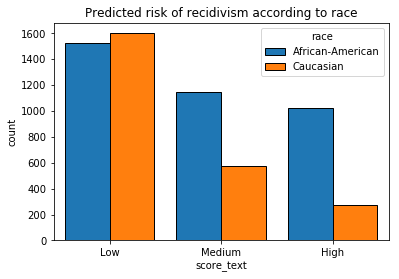
\includegraphics[width=0.5\linewidth]{imgs/predicted_recid_race}
		\caption{It is clear from this illustration that the number of caucasian and african-american people in the low group are almost equal. Meanwhile the medium and high groups contain a much larger fraction of african-americans. Since, in total, there are more african-americans in the dataset than whites (3696/2454), it would seem based purely on the data that whites are more often classified as low risk of recidivism while african-americans are often classified as medium or high risk.}
		\label{fig:predictedrecidrace}
	\end{figure}
	
	\begin{figure}[H]
		\centering
		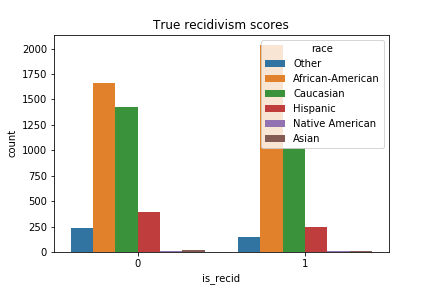
\includegraphics[width=0.5\linewidth]{imgs/true_recid}
		\caption{This illustration shows the true recidivism values (0 being no recidivism after two years and 1 being recidivism) for all offenders in the dataset seperated by the race of each offender. It is clear that close to an equal amount of white and african-american offenders did not recidivate, while a much larger proportion of african-americans re-offended than whites. This makes it difficult to prove bias in the data based only on the data, as it is not necessarily a bias that african-americans more often re-offend.}
		\label{fig:truerecid}
	\end{figure}
	
	\begin{figure}[H]
		\centering
		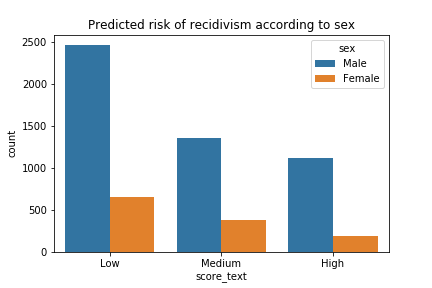
\includegraphics[width=0.5\linewidth]{imgs/predicted_recid_sex}
		\caption{This illustration shows the relationship between sex and the COMPAS prediction of recidivism. The first point to be noted is that there are a lot more men in the dataset than women (5819/1395). Aside from this, it does not seem like there is a difference in the proportions of men or women being classified as belonging to each of the categories.}
		\label{fig:predictedrecidsex}
	\end{figure}
	
	\begin{figure}[H]
		\centering
		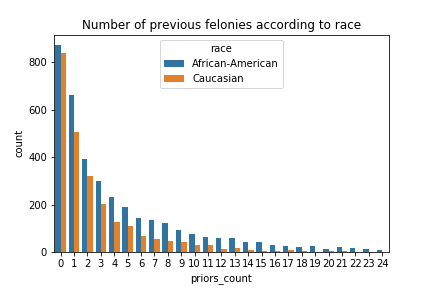
\includegraphics[width=0.5\linewidth]{imgs/proirs}
		\caption{An illustration of the relation between race (african-american or caucasian) and the number of previous felonies prior to the study taking place. This plot gives a clear indication that the number of whites and african-americans who have performed no prior felonies is similar. Otherwise, it is clear that the proportion of african-american to whites becomes larger as the number of previous felonies becomes larger. This seems to indicate that african-americans are more often engaged in criminal activity, which also weakens the indication of a bias from \ref{fig:predictedrecidrace}.}
		\label{fig:proirs}
	\end{figure}
	
	
	
	\subsection{Data ethicality}
	The COMPAS dataset as well as ProPublica's expanded data and analysis of this data is freely available from their public GitHub repository. As such, the data is not stored safely. This is also true for the variables of the data such as age, full name and number of previous felonies, which give ample opportunity to identify people who have recidivated, leading to compromise of their personal data. This is not a concern though, as the data is collected from Florida, where public records are subject to the broad legislated public right of inspection. According to chapter 119 section 1 of the law of the State of Florida, 
	\begin{displayquote}
		"It is the policy of this state that all state, county, and municipal records are open for personal inspection and copying by any person. Providing access to public records is a duty of each agency." \cite{floridaLaw}
	\end{displayquote}
	
	\noindent As such, since ProPublica submitted a public records request for access to the data for use in research \cite{propublicaAnalysis}, which inherently is a type of inspection, they are within the legal ramifications to use the dataset as they please. Another debate entirely, which will in particular be taken up in \ref{discussion}, is the more subjective question of the ethicality of open-record laws and public criminal data in their entirety being shared among whomever and what exactly should be allowed to be done with this data.
	
		
	\section{Methods} \label{methods}
	\textbf{TODO: \\ referér til kode og software \\ brug lang tid på nye metoder, kort tid på gamle metoder}
	
	\subsection{Binary Classifier}\label{Feed-forward neural}
	%initialization schemes
	\subsubsection{Feed-forward Neural Network}
	Feed-forward neural networks (FFNN) are the simplest form of a neural network. Information flow in a feed-forward neural is one directional which means that the network has an input layer, and information flow from these nodes through the hidden layers unto the output layer. The main purpose of a FFNN is to approximate a function. In this project $ y = f^*(x) $ maps an input $ \mathbf x $ to a category $ \mathbf y $. The FFNN is thereby a classifier, which goal is to determine the recidvism risk of a person given the input variable $ \mathbf x $. The input variable $ \mathbf x $ contains \textbf{TODO:}. The categories of $ \mathbf y $ is either 0 or 1, which corresponds to the classifier classifying a person as either low or medium/high risk of recidivism. Hence, this is a binary classifier which constructs a mapping $ \mathbf y = f(\mathbf x \ ; \mathbf w) $. The goal is to learn the weights that most efficiently approximate the function $ f^* $ through supervised learning. The binary classifier in this project has an input layer, three hidden layers and an output layer. \cite{dl}
	
	\begin{figure}[H]
		\centering
		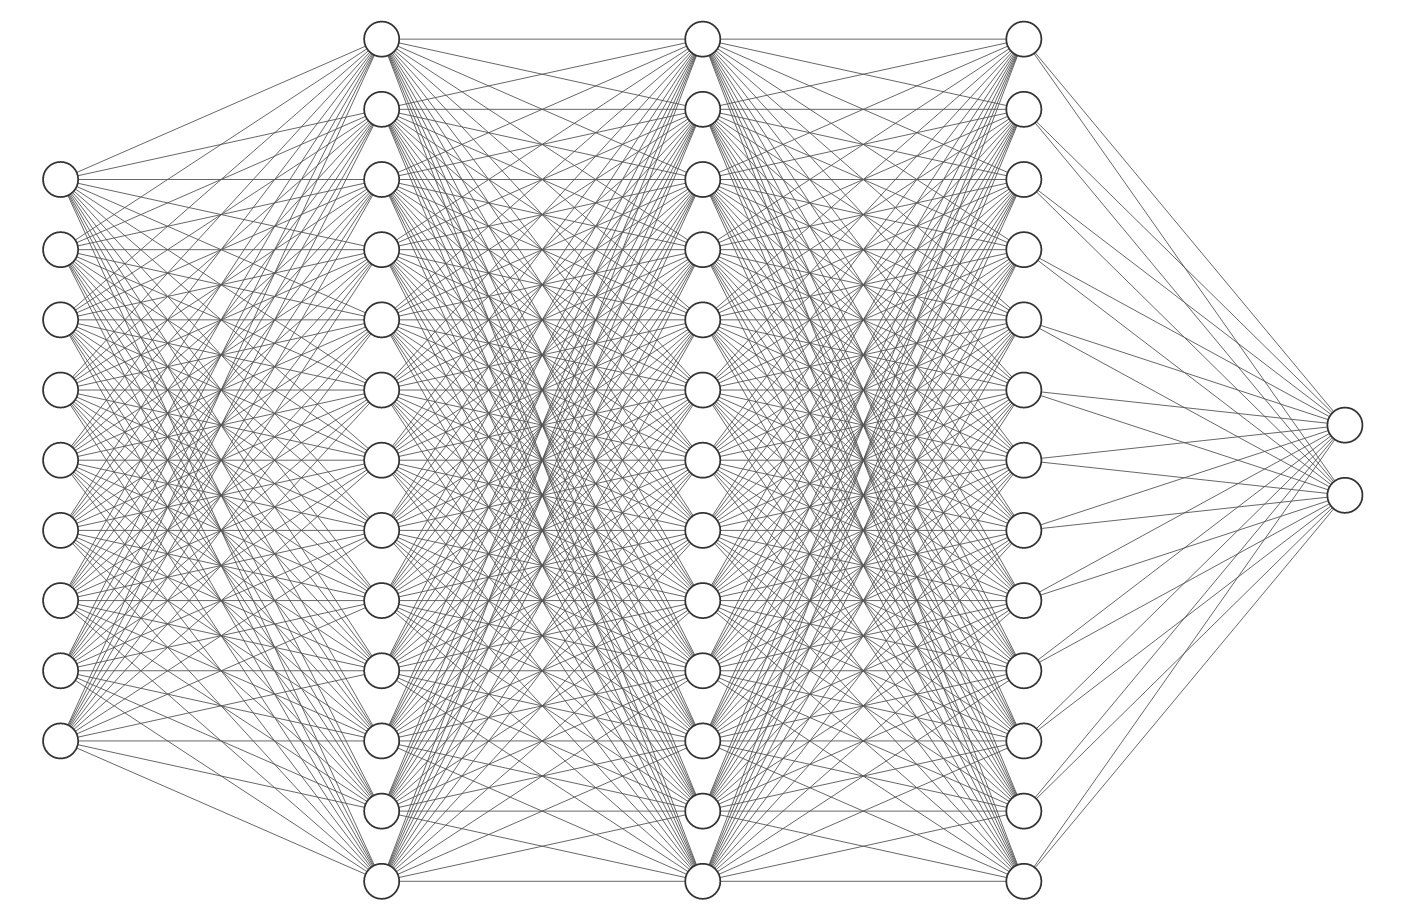
\includegraphics[width=0.5\linewidth]{imgs/ffnn}
		\caption{Visualization of the binary classifier model. The input layer has dimension $ \mathbb R ^9$ and the output layer has dimension $ \mathbb R^2 $. The number of nodes in the hidden layers is a changeable parameter which is found with Bayesian Optimization. }
		\label{fig:ffnn}
	\end{figure}
	
	
	\subsubsection{Bayesian Optimization}
	%Bayesian Optimization
	
	To obtain the pinnacle of accuracy in a neural network, it needs an excellent architecture as well as the potimal hyperparameters. However, the search for these parameters are usually a costly process of uncertainty balancing exploration of parameters and the exploitation of results. Often the process of finding the optimal parameters and network architecture comes from expert knowledge, biased heuristics or exhaustive sampling from the parameter space. To determine the architecture and hyperparameters of the binary classifier Bayesian Optimization is used. 
	\subparagraph*{Objective Function}
	The objective function that is being optimized in this project is the binary classifier presented above. The fully connected layers are trained on the COMPASS data-set and the validation accuracy of the model is what BO optimizes. The accuracy of the constructed model is evaluated using non-parametric Gaussian Process (GP) as a function fo the following hyperparameters:
	\begin{itemize}
		\item Number of units in the first hidden layer \(\in [1, 5000]\) 
		\item Number of units in the second hidden layer \(\in [1, 5000]\) 
		\item Number of units in the third hidden layer \(\in [1, 5000]\)
		\item Dropout probability \(\in [0,1]\)
		\item Activation function \{tanh, ReLU, ReLU6, Sigmoid\}
	\end{itemize}
	The hyperparameters that are not changed are the learning rate, which is set at $ \alpha = 0.001 $. The reason why this parameter is not changed is due to the fact, that the optimizer implemented in this project, is Adaptive Moment Estimation (Adam). Adam is a well known optimizer in the literature and has adaptive learning rate as well as step size. Which is why this learning rate is not an interchangeable hyperparameter. \\ Cross Entropy Loss is used as the cost-function. The loss is in the binary classfier is calculated as the following, 
	\begin{equation}\label{key}
	L\left(\boldsymbol{y}_{i}, \hat{\boldsymbol{y}}_{i}\right) = -(\mathbf y \log (\mathbf {\hat y})+(1-\mathbf  y) \log (1-\mathbf {\hat y}))
	\end{equation}
	The cross entropy loss punishes the algorithm if the predicted value is far from the label. I.e. if the classifier predicts 0.09 and the label is 1, it would result in a very high loss. The ideal model would have a cross entropy loss of zero. The loss function will remain untouched during the Bayesian Optimization. \cite {dl}
	\\\\
	Gaussian Process uses the smoothness assumption on the outputs of the network, and its variance and lengthscale parameters are optimized using maximum log-likelihood principle. \cite{aktiv_gp} The acquisition function, that choose the parameters for the model, used is Expected Improvement (EI). EI attempts to quantify the improvement of the parameters chosen. The average improvement is quantified by sampling the objective function at $x$. The acquisition function then computes the expected value of the improvement function at a certain $x$. EI is expressed as 
	\begin{equation*}
	\mathrm{EI}(\mathbf{x})=\left\{\begin{array}{ll}
	\left(\mu(\mathbf{x})-f\left(\mathbf{x}^{+}\right)\right) \Phi(Z)+\sigma(\mathbf{x}) \phi(Z) & \text { if } \sigma(\mathbf{x})>0 \\
	0 & \text { if } \sigma(\mathbf{x})<0,
	\end{array}\right. 
	\end{equation*}
	where $ Z = \frac{\mu(\mathbf{x}) - f(\mathbf{x}^+) - \xi }{\sigma(\mathbf{x})}$ , \cite{aktiv_bo} 
	\\\\
	The Bayesian Optimization starts by sampling from the objective function, then it fits the Gaussian Process to the sampled points and then iterates the next points in the hyperparameter space using the fitted GP and Expected Improvement. As for the implementation of Baysesian Optimization the GPyOpt library is used \cite{bo_lib}. The exploration / exploitation trade-off variable \textit{jitter} is set to the default value of 0.01.
	
	\subsection{Permutation test}
	To identify whether or not the data-set is biased, and if this has impacted the constructed binary classifier, a permutation test was conducted. A permutation test is a non-parametric test that has no distributional assumption. Permutation tests can also be used to see the importance of a feature in the data-set. Therefore permutation test was used for both feature selection and identification of bias in the binary classifier. \\\\
	As for feature selection every feature was randomly shuffled with re-sampling. If the outputs remained unchanged regardless of the permutation the feature was dropped. Every feature is permuted 1000 times.\\\\
	As for identification of biases in the binary classifier the categorical race was used. Permutation was implemented by randomly shuffling the attribute with re-sampling. The permuted data were used as input for the model and several confusion matrices were constructed and compared. The matrices were compared to the original confusion matrix, which in turn results in a \textit{p}-value on the percentage of false negatives (FN) on whites compared to African-Americans in the ProPublica data.
	
	\subsection{Bias Correction	n Methods}
	
	\section{Results} \label{results}
	\textbf{TODO \\ dokumentér reproducerbarheden af resultaterne \\ tabeller og figurer over resultater \\ forklar resultaterne endten i diskussion eller resultater.}
	
	\section{Discussion} \label{discussion}
	\textbf{TODO: \\ etisk diskussion omkring teknologien der er arbejdet med}
	
	\section{Conclusion} \label{conclusion}
	\textbf{TODO: \\ Opsummér resultater og anbefalinger fra projektet \\ Må ikke indeholde noget nyt \\ Skal svare på spørgsmålene fra problemformuleringen \\ Konklusion, abstract og indledning skal give samlet billede af projektet}
	
	\section{Appendix} \label{appendix}
	
	\begin{figure}[H]
		\centering
		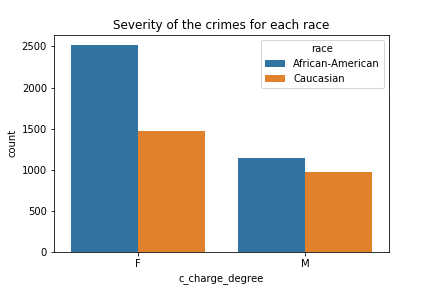
\includegraphics[width=0.5\linewidth]{imgs/c_charge_degree}
		\caption{}
		\label{fig:cchargedegree}
	\end{figure}
	
	\begin{figure}[H]
		\centering
		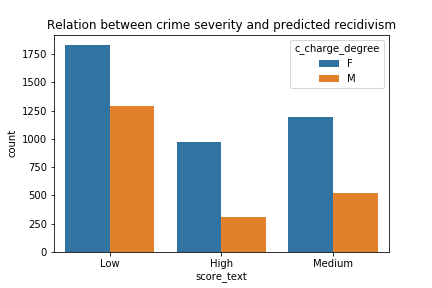
\includegraphics[width=0.5\linewidth]{imgs/charge_degree_score}
		\caption{}
		\label{fig:chargedegreescore}
	\end{figure}
	
	\begin{thebibliography}{9} \label{bibliography}
		
		\bibitem{bo_lib} Machine Learning Group, University of Sheffield: "GPyOpt’s documentation", at \url{https://gpyopt.readthedocs.io}
		
		\bibitem{equal_of_oppor} M. Hardt, E. Price, and N. Srebro. Equality of Opportunity in Supervised Learning. In NIPS, 2016.
		
		\bibitem{Zafar} M. B. Zafar, I. Valera, M. G. Rodriguez, and K. P. Gummadi. Fairness constraints: A mechanism for fair classification.
		In ICML Workshop on Fairness, Accountability, and Transparency in Machine Learning, 2015.
		
		\bibitem{floridaLaw} The State of Florida, "The 2019 Florida Statutes", 1995,  \url{http://www.leg.state.fl.us/statutes/index.cfm?App_mode=Display_Statute&URL=0100-0199/0119/0119.html}, visited 12-03-2020
		
		\bibitem{propublicaAnalysis} ProPublica, "How We Analyzed the COMPAS Recidivism Algorithm", 2016, \url{https://www.propublica.org/article/how-we-analyzed-the-compas-recidivism-algorithm}, visited 12-03-2020
		
		\bibitem{aktiv_gp} F. Bergamin. 02463 “Active Machine Learning and Agency” Lecture 1: Gaussian Processes, 2020.
		
		\bibitem{aktiv_bo} F. Bergamin. 02463 “Active Machine Learning and Agency” Lecture 2: Bayesian Optimization, 2020.
		
		\bibitem{dl} Goodfellow-et-al-2016. Deep Learning, MIT Press in 2016. 
		
		\bibitem{b_woodworth} B. Woodworth et al. Learning Non-Discriminatory Predictors, Toyota Technological Institute at Chicago, Chicago, IL 60637, USA.
		
		\bibitem{g_goh} G. Goh et al. Satisfying Real-world Goals with Dataset Constraints. In NIPS, 2016.
		
	\end{thebibliography}
	
	\newpage
	\bibliographystyle{IEEEbib}
	\bibliography{refs}
\end{document}
